
%% bare_jrnl.tex
%% V1.4a
%% 2014/09/17
%% by Michael Shell
%% see http://www.michaelshell.org/
%% for current contact information.
%%
%% This is a skeleton file demonstrating the use of IEEEtran.cls
%% (requires IEEEtran.cls version 1.8a or later) with an IEEE
%% journal paper.
%%
%% Support sites:
%% http://www.michaelshell.org/tex/ieeetran/
%% http://www.ctan.org/tex-archive/macros/latex/contrib/IEEEtran/
%% and
%% http://www.ieee.org/

%%*************************************************************************
%% Legal Notice:
%% This code is offered as-is without any warranty either expressed or
%% implied; without even the implied warranty of MERCHANTABILITY or
%% FITNESS FOR A PARTICULAR PURPOSE! 
%% User assumes all risk.
%% In no event shall IEEE or any contributor to this code be liable for
%% any damages or losses, including, but not limited to, incidental,
%% consequential, or any other damages, resulting from the use or misuse
%% of any information contained here.
%%
%% All comments are the opinions of their respective authors and are not
%% necessarily endorsed by the IEEE.
%%
%% This work is distributed under the LaTeX Project Public License (LPPL)
%% ( http://www.latex-project.org/ ) version 1.3, and may be freely used,
%% distributed and modified. A copy of the LPPL, version 1.3, is included
%% in the base LaTeX documentation of all distributions of LaTeX released
%% 2003/12/01 or later.
%% Retain all contribution notices and credits.
%% ** Modified files should be clearly indicated as such, including  **
%% ** renaming them and changing author support contact information. **
%%
%% File list of work: IEEEtran.cls, IEEEtran_HOWTO.pdf, bare_adv.tex,
%%                    bare_conf.tex, bare_jrnl.tex, bare_conf_compsoc.tex,
%%                    bare_jrnl_compsoc.tex, bare_jrnl_transmag.tex
%%*************************************************************************


% *** Authors should verify (and, if needed, correct) their LaTeX system  ***
% *** with the testflow diagnostic prior to trusting their LaTeX platform ***
% *** with production work. IEEE's font choices and paper sizes can       ***
% *** trigger bugs that do not appear when using other class files.       ***                          ***
% The testflow support page is at:
% http://www.michaelshell.org/tex/testflow/



\documentclass[journal]{IEEEtran}
%
% If IEEEtran.cls has not been installed into the LaTeX system files,
% manually specify the path to it like:
% \documentclass[journal]{../sty/IEEEtran}


\usepackage{amsmath,graphicx}
\usepackage{amsfonts}
\usepackage{bm}
\usepackage{amsthm}
\newtheorem{proposition}{Proposition}



% Some very useful LaTeX packages include:
% (uncomment the ones you want to load)


% *** MISC UTILITY PACKAGES ***
%
%\usepackage{ifpdf}
% Heiko Oberdiek's ifpdf.sty is very useful if you need conditional
% compilation based on whether the output is pdf or dvi.
% usage:
% \ifpdf
%   % pdf code
% \else
%   % dvi code
% \fi
% The latest version of ifpdf.sty can be obtained from:
% http://www.ctan.org/tex-archive/macros/latex/contrib/oberdiek/
% Also, note that IEEEtran.cls V1.7 and later provides a builtin
% \ifCLASSINFOpdf conditional that works the same way.
% When switching from latex to pdflatex and vice-versa, the compiler may
% have to be run twice to clear warning/error messages.






% *** CITATION PACKAGES ***
%
%\usepackage{cite}
% cite.sty was written by Donald Arseneau
% V1.6 and later of IEEEtran pre-defines the format of the cite.sty package
% \cite{} output to follow that of IEEE. Loading the cite package will
% result in citation numbers being automatically sorted and properly
% "compressed/ranged". e.g., [1], [9], [2], [7], [5], [6] without using
% cite.sty will become [1], [2], [5]--[7], [9] using cite.sty. cite.sty's
% \cite will automatically add leading space, if needed. Use cite.sty's
% noadjust option (cite.sty V3.8 and later) if you want to turn this off
% such as if a citation ever needs to be enclosed in parenthesis.
% cite.sty is already installed on most LaTeX systems. Be sure and use
% version 5.0 (2009-03-20) and later if using hyperref.sty.
% The latest version can be obtained at:
% http://www.ctan.org/tex-archive/macros/latex/contrib/cite/
% The documentation is contained in the cite.sty file itself.






% *** GRAPHICS RELATED PACKAGES ***
%
\ifCLASSINFOpdf
  % \usepackage[pdftex]{graphicx}
  % declare the path(s) where your graphic files are
  % \graphicspath{{../pdf/}{../jpeg/}}
  % and their extensions so you won't have to specify these with
  % every instance of \includegraphics
  % \DeclareGraphicsExtensions{.pdf,.jpeg,.png}
\else
  % or other class option (dvipsone, dvipdf, if not using dvips). graphicx
  % will default to the driver specified in the system graphics.cfg if no
  % driver is specified.
  % \usepackage[dvips]{graphicx}
  % declare the path(s) where your graphic files are
  % \graphicspath{{../eps/}}
  % and their extensions so you won't have to specify these with
  % every instance of \includegraphics
  % \DeclareGraphicsExtensions{.eps}
\fi
% graphicx was written by David Carlisle and Sebastian Rahtz. It is
% required if you want graphics, photos, etc. graphicx.sty is already
% installed on most LaTeX systems. The latest version and documentation
% can be obtained at: 
% http://www.ctan.org/tex-archive/macros/latex/required/graphics/
% Another good source of documentation is "Using Imported Graphics in
% LaTeX2e" by Keith Reckdahl which can be found at:
% http://www.ctan.org/tex-archive/info/epslatex/
%
% latex, and pdflatex in dvi mode, support graphics in encapsulated
% postscript (.eps) format. pdflatex in pdf mode supports graphics
% in .pdf, .jpeg, .png and .mps (metapost) formats. Users should ensure
% that all non-photo figures use a vector format (.eps, .pdf, .mps) and
% not a bitmapped formats (.jpeg, .png). IEEE frowns on bitmapped formats
% which can result in "jaggedy"/blurry rendering of lines and letters as
% well as large increases in file sizes.
%
% You can find documentation about the pdfTeX application at:
% http://www.tug.org/applications/pdftex





% *** MATH PACKAGES ***
%
%\usepackage[cmex10]{amsmath}
% A popular package from the American Mathematical Society that provides
% many useful and powerful commands for dealing with mathematics. If using
% it, be sure to load this package with the cmex10 option to ensure that
% only type 1 fonts will utilized at all point sizes. Without this option,
% it is possible that some math symbols, particularly those within
% footnotes, will be rendered in bitmap form which will result in a
% document that can not be IEEE Xplore compliant!
%
% Also, note that the amsmath package sets \interdisplaylinepenalty to 10000
% thus preventing page breaks from occurring within multiline equations. Use:
%\interdisplaylinepenalty=2500
% after loading amsmath to restore such page breaks as IEEEtran.cls normally
% does. amsmath.sty is already installed on most LaTeX systems. The latest
% version and documentation can be obtained at:
% http://www.ctan.org/tex-archive/macros/latex/required/amslatex/math/





% *** SPECIALIZED LIST PACKAGES ***
%
%\usepackage{algorithmic}
% algorithmic.sty was written by Peter Williams and Rogerio Brito.
% This package provides an algorithmic environment fo describing algorithms.
% You can use the algorithmic environment in-text or within a figure
% environment to provide for a floating algorithm. Do NOT use the algorithm
% floating environment provided by algorithm.sty (by the same authors) or
% algorithm2e.sty (by Christophe Fiorio) as IEEE does not use dedicated
% algorithm float types and packages that provide these will not provide
% correct IEEE style captions. The latest version and documentation of
% algorithmic.sty can be obtained at:
% http://www.ctan.org/tex-archive/macros/latex/contrib/algorithms/
% There is also a support site at:
% http://algorithms.berlios.de/index.html
% Also of interest may be the (relatively newer and more customizable)
% algorithmicx.sty package by Szasz Janos:
% http://www.ctan.org/tex-archive/macros/latex/contrib/algorithmicx/




% *** ALIGNMENT PACKAGES ***
%
%\usepackage{array}
% Frank Mittelbach's and David Carlisle's array.sty patches and improves
% the standard LaTeX2e array and tabular environments to provide better
% appearance and additional user controls. As the default LaTeX2e table
% generation code is lacking to the point of almost being broken with
% respect to the quality of the end results, all users are strongly
% advised to use an enhanced (at the very least that provided by array.sty)
% set of table tools. array.sty is already installed on most systems. The
% latest version and documentation can be obtained at:
% http://www.ctan.org/tex-archive/macros/latex/required/tools/


% IEEEtran contains the IEEEeqnarray family of commands that can be used to
% generate multiline equations as well as matrices, tables, etc., of high
% quality.




% *** SUBFIGURE PACKAGES ***
%\ifCLASSOPTIONcompsoc
%  \usepackage[caption=false,font=normalsize,labelfont=sf,textfont=sf]{subfig}
%\else
%  \usepackage[caption=false,font=footnotesize]{subfig}
%\fi
% subfig.sty, written by Steven Douglas Cochran, is the modern replacement
% for subfigure.sty, the latter of which is no longer maintained and is
% incompatible with some LaTeX packages including fixltx2e. However,
% subfig.sty requires and automatically loads Axel Sommerfeldt's caption.sty
% which will override IEEEtran.cls' handling of captions and this will result
% in non-IEEE style figure/table captions. To prevent this problem, be sure
% and invoke subfig.sty's "caption=false" package option (available since
% subfig.sty version 1.3, 2005/06/28) as this is will preserve IEEEtran.cls
% handling of captions.
% Note that the Computer Society format requires a larger sans serif font
% than the serif footnote size font used in traditional IEEE formatting
% and thus the need to invoke different subfig.sty package options depending
% on whether compsoc mode has been enabled.
%
% The latest version and documentation of subfig.sty can be obtained at:
% http://www.ctan.org/tex-archive/macros/latex/contrib/subfig/




% *** FLOAT PACKAGES ***
%
%\usepackage{fixltx2e}
% fixltx2e, the successor to the earlier fix2col.sty, was written by
% Frank Mittelbach and David Carlisle. This package corrects a few problems
% in the LaTeX2e kernel, the most notable of which is that in current
% LaTeX2e releases, the ordering of single and double column floats is not
% guaranteed to be preserved. Thus, an unpatched LaTeX2e can allow a
% single column figure to be placed prior to an earlier double column
% figure. The latest version and documentation can be found at:
% http://www.ctan.org/tex-archive/macros/latex/base/


%\usepackage{stfloats}
% stfloats.sty was written by Sigitas Tolusis. This package gives LaTeX2e
% the ability to do double column floats at the bottom of the page as well
% as the top. (e.g., "\begin{figure*}[!b]" is not normally possible in
% LaTeX2e). It also provides a command:
%\fnbelowfloat
% to enable the placement of footnotes below bottom floats (the standard
% LaTeX2e kernel puts them above bottom floats). This is an invasive package
% which rewrites many portions of the LaTeX2e float routines. It may not work
% with other packages that modify the LaTeX2e float routines. The latest
% version and documentation can be obtained at:
% http://www.ctan.org/tex-archive/macros/latex/contrib/sttools/
% Do not use the stfloats baselinefloat ability as IEEE does not allow
% \baselineskip to stretch. Authors submitting work to the IEEE should note
% that IEEE rarely uses double column equations and that authors should try
% to avoid such use. Do not be tempted to use the cuted.sty or midfloat.sty
% packages (also by Sigitas Tolusis) as IEEE does not format its papers in
% such ways.
% Do not attempt to use stfloats with fixltx2e as they are incompatible.
% Instead, use Morten Hogholm'a dblfloatfix which combines the features
% of both fixltx2e and stfloats:
%
% \usepackage{dblfloatfix}
% The latest version can be found at:
% http://www.ctan.org/tex-archive/macros/latex/contrib/dblfloatfix/




%\ifCLASSOPTIONcaptionsoff
%  \usepackage[nomarkers]{endfloat}
% \let\MYoriglatexcaption\caption
% \renewcommand{\caption}[2][\relax]{\MYoriglatexcaption[#2]{#2}}
%\fi
% endfloat.sty was written by James Darrell McCauley, Jeff Goldberg and 
% Axel Sommerfeldt. This package may be useful when used in conjunction with 
% IEEEtran.cls'  captionsoff option. Some IEEE journals/societies require that
% submissions have lists of figures/tables at the end of the paper and that
% figures/tables without any captions are placed on a page by themselves at
% the end of the document. If needed, the draftcls IEEEtran class option or
% \CLASSINPUTbaselinestretch interface can be used to increase the line
% spacing as well. Be sure and use the nomarkers option of endfloat to
% prevent endfloat from "marking" where the figures would have been placed
% in the text. The two hack lines of code above are a slight modification of
% that suggested by in the endfloat docs (section 8.4.1) to ensure that
% the full captions always appear in the list of figures/tables - even if
% the user used the short optional argument of \caption[]{}.
% IEEE papers do not typically make use of \caption[]'s optional argument,
% so this should not be an issue. A similar trick can be used to disable
% captions of packages such as subfig.sty that lack options to turn off
% the subcaptions:
% For subfig.sty:
% \let\MYorigsubfloat\subfloat
% \renewcommand{\subfloat}[2][\relax]{\MYorigsubfloat[]{#2}}
% However, the above trick will not work if both optional arguments of
% the \subfloat command are used. Furthermore, there needs to be a
% description of each subfigure *somewhere* and endfloat does not add
% subfigure captions to its list of figures. Thus, the best approach is to
% avoid the use of subfigure captions (many IEEE journals avoid them anyway)
% and instead reference/explain all the subfigures within the main caption.
% The latest version of endfloat.sty and its documentation can obtained at:
% http://www.ctan.org/tex-archive/macros/latex/contrib/endfloat/
%
% The IEEEtran \ifCLASSOPTIONcaptionsoff conditional can also be used
% later in the document, say, to conditionally put the References on a 
% page by themselves.




% *** PDF, URL AND HYPERLINK PACKAGES ***
%
%\usepackage{url}
% url.sty was written by Donald Arseneau. It provides better support for
% handling and breaking URLs. url.sty is already installed on most LaTeX
% systems. The latest version and documentation can be obtained at:
% http://www.ctan.org/tex-archive/macros/latex/contrib/url/
% Basically, \url{my_url_here}.




% *** Do not adjust lengths that control margins, column widths, etc. ***
% *** Do not use packages that alter fonts (such as pslatex).         ***
% There should be no need to do such things with IEEEtran.cls V1.6 and later.
% (Unless specifically asked to do so by the journal or conference you plan
% to submit to, of course. )


% correct bad hyphenation here
\hyphenation{}


\begin{document}
%
% paper title
% Titles are generally capitalized except for words such as a, an, and, as,
% at, but, by, for, in, nor, of, on, or, the, to and up, which are usually
% not capitalized unless they are the first or last word of the title.
% Linebreaks \\ can be used within to get better formatting as desired.
% Do not put math or special symbols in the title.
\title{Modulation Design in Amplify-and-Forward Two-Way Relay HARQ Channel}
%
%
% author names and IEEE memberships
% note positions of commas and nonbreaking spaces ( ~ ) LaTeX will not break
% a structure at a ~ so this keeps an author's name from being broken across
% two lines.
% use \thanks{} to gain access to the first footnote area
% a separate \thanks must be used for each paragraph as LaTeX2e's \thanks
% was not built to handle multiple paragraphs
%

\author{
  Author,~\IEEEmembership{Member,~IEEE,}
  \thanks{}% <-this % stops a space
}

% note the % following the last \IEEEmembership and also \thanks - 
% these prevent an unwanted space from occurring between the last author name
% and the end of the author line. i.e., if you had this:
% 
% \author{....lastname \thanks{...} \thanks{...} }
%                     ^------------^------------^----Do not want these spaces!
%
% a space would be appended to the last name and could cause every name on that
% line to be shifted left slightly. This is one of those "LaTeX things". For
% instance, "\textbf{A} \textbf{B}" will typeset as "A B" not "AB". To get
% "AB" then you have to do: "\textbf{A}\textbf{B}"
% \thanks is no different in this regard, so shield the last } of each \thanks
% that ends a line with a % and do not let a space in before the next \thanks.
% Spaces after \IEEEmembership other than the last one are OK (and needed) as
% you are supposed to have spaces between the names. For what it is worth,
% this is a minor point as most people would not even notice if the said evil
% space somehow managed to creep in.



% The paper headers
\markboth{Journal of \LaTeX\ Class Files,~Vol.~13, No.~9, September~2014}%
{Shell \MakeLowercase{\textit{et al.}}: Bare Demo of IEEEtran.cls for Journals}
% The only time the second header will appear is for the odd numbered pages
% after the title page when using the twoside option.
% 
% *** Note that you probably will NOT want to include the author's ***
% *** name in the headers of peer review papers.                   ***
% You can use \ifCLASSOPTIONpeerreview for conditional compilation here if
% you desire.




% If you want to put a publisher's ID mark on the page you can do it like
% this:
%\IEEEpubid{0000--0000/00\$00.00~\copyright~2014 IEEE}
% Remember, if you use this you must call \IEEEpubidadjcol in the second
% column for its text to clear the IEEEpubid mark.



% use for special paper notices
%\IEEEspecialpapernotice{(Invited Paper)}




% make the title area
\maketitle

% As a general rule, do not put math, special symbols or citations
% in the abstract or keywords.
\begin{abstract}
% (what we do)
  As a practical transmission enhancement technique for relay and HARQ system,
  Modulation Diversity (MoDiv) uses distinct mappings from information bits to
  the same constellation for different (re)transmissions. 
  % (how they do)
  % (how we do)
  In this work, we study the MoDiv optimization
  in a amplify-and-forward (AF) two-way relay channel (TWRC). The design of
  MoDiv design to minimize the bit-error rate (BER) is formulated into a
  successive Koopmans-Beckmann Quadratic Assignment Problem (QAP), which is solved
  sequatially with a robust taboo search method.
  % (main results)
  The performance gain of our MoDiv scheme over retransmission without remapping
  and a heuristic MoDiv scheme is demonstrated with numerical ressults.
\end{abstract}

% Note that keywords are not normally used for peerreview papers.
\begin{IEEEkeywords}
  Modulation diversity, two-way relay, amplify-and-forward, HARQ, QAP.
\end{IEEEkeywords}






% For peer review papers, you can put extra information on the cover
% page as needed:
% \ifCLASSOPTIONpeerreview
% \begin{center} \bfseries EDICS Category: 3-BBND \end{center}
% \fi
%
% For peerreview papers, this IEEEtran command inserts a page break and
% creates the second title. It will be ignored for other modes.
\IEEEpeerreviewmaketitle



\section{Introduction}
\label{sec:intro}

% Motivation and literature review for Two-way relay-HARQ. HARQ first,
% then two-way relay
\IEEEPARstart{A}{s} an advanced technique to improve the robustness of high-rate wireless
transmissions against poor channel conditions, Hybrid Automatic Repeat reQuest
(HARQ) has been widely adopted in various communication
systems~\cite{cripriano2010overview}. HARQ works on both PHY layer and MAC
sublayer to mitigate packet loss due to channel fading and
link-adaptation accuracy. Recently, there has been some research interests in
applying HARQ over two-way relay channel (TWRC) [2-4].
In~\cite{iannello2009throughput}, the average throughput of a simple Type-I HARQ
policy for both Amplify-and-Forward (AF) and Decode-and-Forward (DF) TWRC
schemes have been analyzed. The energy-delay tradeoff, and the diversity-multiplexing
tradeoff of type-II HARQ policy, also known as full Incremental Redundancy (IR),
for AF TWRC scheme have been studied in~\cite{choi2013energy}
and~\cite{xu2014diversity}, respectively. Related works on TWRC with ARQ
for different relay schemes and retransmission policies can also be
found in~\cite{popovski2007wireless, chen2012arq, guan2015twoway} and the references therein.

% Literature review on MoDiv for HARQ-CC
Apart from Type-I HARQ and HARQ-IR, Type-I HARQ with maximal ratio
combining (MRC), also known as HARQ-Chase Combining
(HARQ-CC)~\cite{chase1985code}, is another simple and effective HARQ
scheme supported by such standands as HSPA~\cite{TS25.308},
LTE~\cite{sesia2009lte}, among others. As practical transmissions often admit
linear modulations of finite-alphabet constellation (e.g. Q-ary QAM), the
performance of HARQ-CC can be improved with Modulation Diversity
(MoDiv)~\cite{benelli1992new}, in which a same group of $\log_2Q$
information bits are mapped to different symbols in a same constellation in
different round of (re)transmissions. MoDiv has been studied for
HARQ~\cite{harvind2005symbol}, relay
networks~\cite{seddik2008trans, khormuji2008rate} and relay-HARQ
systems~\cite{kim2009design, ryu2011ber}.

% What we are studying
In this paper, we study the MoDiv design for the TWRC under a simple AF scheme
and HARQ-CC protocol. We first derive an approximation for the uncoded bit-error
rate (BER) of TWRC-AF channel under Rayleigh fading channel condition, given $M$
different mapping schemes corresponding to each (re)transmission. Based on this
approximation, we formulate a successive BER minimization MoDiv design into a
series of Quadratic Assignment Problem (QAP) in Koopmans-Beckmann (KB)
form~\cite{koopmans1957assignment}. Although QAP is NP-hard, efficient numerical
algorithms have been extensively researched~\cite{benlic2015memetic}, some of
which have shown extremely high performance over
QAPLIB~\cite{burkard1997qaplib}. We adopt a taboo search
algorithm~\cite{taillard1991robust} to solve each QAP in our formulation. Moreover, the coefficients of QAP problem can be also be computed efficiently in a
successive manner based on the solution to the preceding QAP problem. Our
numerical results demonstrate significant BER reduction over both non-MoDiv and
a simple heuristic MoDiv retransmission scheme for 16-QAM and 64-QAM
constellations, even under mismatched design parameters.

% Structure of the manuscript
The paper is organized as follows. Section~\ref{sec:model} introduces the
TWRC-AF model and the HARQ protocol we are using. Section~\ref{sec:modiv}
presents the successive BER minimization MoDiv design problem. In
Section~\ref{sec:numerical}, we present the numerical results to show the
performance gain of our MoDiv scheme. Finally, Section~\ref{sec:conclusion}
concludes the paper.


% needed in second column of first page if using \IEEEpubid
%\IEEEpubidadjcol

\section{System Model}
\label{sec:model}

% Two-way relay channel
Consider a TWRC with analog network coding (ANC) protocol~\cite{choi2013energy}, 
a generalization the AF protocol, as shown in Fig.~\ref{fig:model}. The relay
node $R$ is totally unaware of the HARQ procedure and simply performs ANC. Each round of ANC
transmission consists of two phases. In the multiple access (MAC) phase, the
two source nodes $S_1$ and $S_2$ transmit to $R$ simultaneously. In the
broadcast (BC) phase, node $R$ amplifies and broadcasts the signal received
during the MAC phase to both $S_1$ and $S_2$.
Denote the uplink channel from $S_s$ to $R$ and downlink channel from $R$ to
$S_s$ as $h_s$ and $g_s$, respectively, where $s=1,2$. We assume that all
the channels follow Rayleigh distribution, i.e.
$h_s\sim\mathcal{CN}(0,\beta_{h_s})$ and $g_s\sim\mathcal{CN}(0,\beta_{g_s})$,
$s=1,2$. Denote the transmitted symbol from $S_s$ as $x_s$ whose average power
$\mathbb{E}[|x_s|^2]=P_s$. Then the signal received by $R$ during the MAC phase
is
\begin{align}
  y_R & = h_1x_1+h_2x_2+n_R,
  \label{eq:y_R}
\end{align}
where $n_R\sim\mathcal{CN}(0,\sigma_R^2)$ is the received noise at $R$. Assuming
that the relay $R$ has an expected power constraint of $P_R$, and that
$S_1$ and $S_2$ perform perfect self-interference cancellation (SIC), then the
received signal at $S_s$ after SIC is
\begin{align}
  y_s &= \alpha g_s y_R + n_s,\;s=1,2,
  \label{eq:y_s}
\end{align}
where $n_s\sim\mathcal{CN}(0,\sigma_s^2)$ is the received noise at $S_s$, and
\begin{align}
  \alpha = \sqrt{\frac{P_R}{|h_1|^2P_1 + |h_2|^2P_2+\sigma_R^2}}
\end{align}
is the power normalization factor at $R$.

% HARQ protocol
On top of this settings, $S_1$ and $S_2$ performs the HARQ-CC protocol
in an unsynchronized manner. Consequently, the MoDiv design at $S_1$ and $S_2$
can be handled independently. Without loss of generality, we study the HARQ
transmission from $S_1$ to $S_2$. Denote $\mathcal{C}$ as the constellation used
by $S_1$ whose cardinality equals $Q=|\mathcal{C}|$. As a convention, during the
initial transmission of a packet, $S_1$ converts a bit sequence of length
$\log_2Q$ into symbols with Gray mapping $\psi_0:\{0,\ldots,Q - 1\}\rightarrow
\mathcal{C}$. The bit sequence is is labeled by its decimal equivalence $p\in
\{0,\ldots,Q - 1\}$. What distinct HARQ-CC with MoDiv from conventional HARQ-CC
is that, during the $m$-th retransmission, $S_1$ is allowed to use a
mapping function $\psi_m\not=\psi_0$ to remap the same label $p$. We assume
$m \leq M$ where $M$ is the maximum number of retransmissions. According to
Eqs.~(\ref{eq:y_R})(\ref{eq:y_s}), the signal received by $S_2$ after SIC during
the $m$-th (re)transmission of $p$ is
\begin{equation}
  y_2^{(m)} = \alpha^{(m)} g_2^{(m)}h_1^{(m)}\psi_m[p] +
  \alpha^{(m)} g_2^{(m)}n_R^{(m)} + n_2^{(m)},
\end{equation}
where $X^{(m)}$ is the $m$-th realization of random variable $X$.

% ML detector
Assume that $S_2$ acquires perfect channel state information
(CSI). After the $m$-th retransmission, it attempts to demodulate the received symbols by
identifying label $p$ with $y_2^{(0)},\ldots,y_2^{(m)}$ via the maximum
likelihood (ML) detection:
\begin{align}
  p^* = \arg\min_p\sum_{k=0}^{m} \frac{|y_2^{(k)} -
  \alpha^{(k)} g_2^{(k)} h_1^{(k)}\psi_k[p]|^2}
  {\sigma_2^2+(\alpha^{(k)})^2\sigma_R^2|g_2^{(k)}|^2}.
  \label{eq:ml}
\end{align}

\begin{figure}[!t]
  \centering
  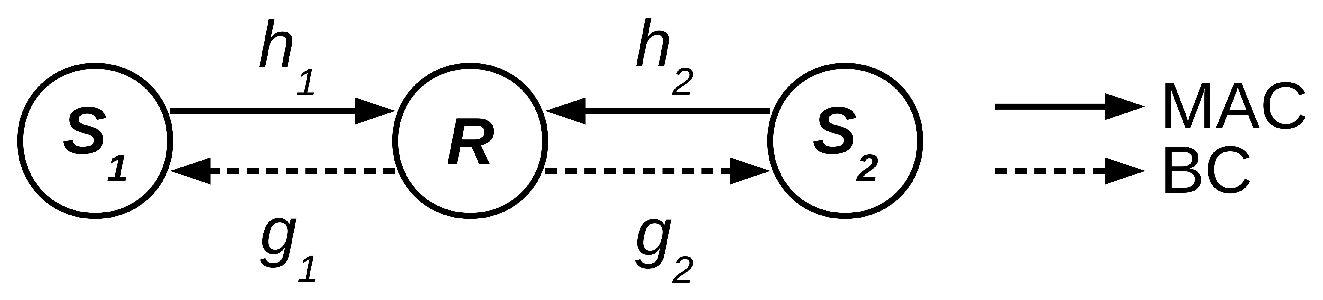
\includegraphics[width=2.0in]{./figs/model.eps}
  \caption{Two-way relay channel with analog network coding.}
  \label{fig:model}
\end{figure}

\section{Successive Constellation Mapping Design For Modulation Diversity}
\label{sec:modiv}
% Outline
In this section, we first derive an closed-form approximation of
the reception bit-error rate in our TWRC channel with HARQ-CC. Based on this
result, we formulate the BER-minimization MoDiv design into a successive
QAP (S-QAP).

\subsection{A BER approximation}
\label{ssec:ber}
% The approximation of BER using PEP
Assume that the label $p$ follows a uniform distribution. The BER of
the ML demodulator after the $m$-th retransmission can be upper-bounded and
approximated with the pair-wise error probability (PEP)~\cite{harvind2005symbol}:
\begin{align}
  P_{BER}^{(m)} = \sum_{p=0}^{Q - 1}\sum_{q=0}^{Q - 1}\frac{B[p,
  q]}{Q}P_{PEP}^{(m)}(q|p), \label{eq:P_BER}
\end{align}
where $B[p,q]$ represents the Hamming distance between the binary representation
of $p$ and $q$ normalized by $\log_2Q$, and $P_{PEP}^{(m)}(q|p)$ is the
probability that the ML demodulator prefer $q$ over $p$ conditioned on the
transmission of $p$. From Eq.~(\ref{eq:ml}), we have
\begin{align}
  P_{PEP}^{(m)}(q|p) = \mathbb{E}
  \left[Q\left(\sqrt{\sum_{k=0}^m \frac{(\alpha^{(k)})^2\epsilon_k[p,q]
  \gamma_2^{(k)} \delta_1^{(k)}} {2(\tilde{\sigma}_2^{(k)})^2}}\right)\right],
  \label{eq:PEP_m}
\end{align}
where $\gamma_2^{(k)} = \|g_2^{(k)}\|^2$, $\delta_1^{(k)} = \|h_1^{(k)}\|^2$
, $\epsilon_k[p,q] = \|\psi_k[p]-\psi_k[q]\|^2$, and $(\tilde{\sigma}_2^{(k)})^2
= \sigma_2^2+(\alpha^{(k)})^2\sigma_R^2\gamma_2^{(k)}$ is the instantaneous
variance of the noise received by $S_2$. By adopting the Chernoff upper bound
$Q(x)\leq e^{-x^2/2}/2$~\cite{proakisdigital}, an approximation to
$P_{PEP}^{(m)}(q|p)$ is
\begin{align}
  \tilde{P}_{PEP}^{(m)}(q|p) = \frac{1}{2}\prod_{k=0}^{m} \mathbb{E}
  \left[\exp\left( 
  -\frac{(\alpha^{(k)})^2\epsilon_k[p,q]\gamma_2^{(k)} \delta_1^{(k)}}
  {4(\tilde{\sigma}_2^{(k)})^2}
  \right)\right].
  \label{eq:PEP_m_approx}
\end{align}
Although the Chernoff bound is a rather coarse appoximation, it
enables efficient iterative computation of $P_{PEP}^{(m)}(q|p)$ as $m$ varies.
Moreover, as shown in Section~\ref{ssec:qap}, this approximation results in a
simple KB-form QAP. Nevertheless, the Chernoff bound can be replaced
with a more accurate approximation as in Eq.(14) of~\cite{chiani2003new},
As will be explained in Section~\ref{ssec:qap}, however, this will lead to a
more complex general-form QAP.

Denote $E_k[p,q]$ as the expectation in Eq.(\ref{eq:PEP_m_approx}), which can be
evaluated as follows:
\begin{proposition}
  An approximation to $E_k[p,q]$ is
  \begin{align}
    \tilde{E}_k[p,q] = \frac{4\sigma_R^2
    + \beta_{h_1}\epsilon_k[p,q]v\exp(v)Ei(v)}{u}
    \label{eq:E_k}
  \end{align}
  where
  \begin{subequations}
    \begin{align}
      u & = 4\sigma_R^2 + \beta_{h_1}\epsilon_k[p,q],\;
      v =
      \frac{4\sigma_2^2}{\tilde{\alpha}^2\beta_{g_2}u}, \notag\\
      \tilde{\alpha} & = \sqrt{\frac{P_R}{\beta_{h_1}P_1 +
      \beta_{h_2}P_2+\sigma_R^2}}, \notag
    \end{align}
  \end{subequations}
  and $Ei(x) = \int_x^\infty e^{-t}/tdt$ is the exponential integral
  function~\cite{zwillinger2014table}. 
  \label{prop:E_k}
\end{proposition}
\begin{proof}
  See Appendix.
\end{proof}
While $E_k[p,q]$ plays a key role in our MoDiv design based on BER minimization,
we comment that it is also closely related to another performance metric, the
ergodic mutual information (EMI), via the following proposition. 
\begin{proposition}
  The EMI after the $m$-th retransmission,
  denoted as $I^{(m)}$, is lower bounded by
  \begin{align}
    \tilde{I}^{(m)} = \log_2Q -
    \log_2\left[ \frac{1}{Q} \sum_{p=0}^{Q-1}\sum_{q=0}^{Q-1}
    \prod_{k=0}^{m}E_k[p,q] \right].
  \end{align}
  \label{prop:EMI}
\end{proposition}
\begin{proof}
  See Appendix.
\end{proof}
Proposition 2 bridges MoDiv design based on rate
criterion~\cite{khormuji2008rate} and BER criterion~\cite{harvind2005symbol}.
Moreover, it leads to an efficient KB-form QAP almost identical to that derived
from the BER minimization, as will be explained in Section~\ref{ssec:qap}.
% Recursion of the approximated PEP

\subsection{The Successive Quadratic Assignment Problem}
\label{ssec:qap}
% Approximated BER minimization
Our MoDiv design is based on the approximated BER minimization criterion. As it
is impossible to know the number of actual retransmission $m$ in advance, we
formulate a sequence of $M$ optimization problems as
in~\cite{harvind2005symbol}, in which $\psi_m$ is optimized to minimize the
approximated BER given $\psi_1,\ldots,\psi_{m-1}$ without expecting future
retransmissions:
\begin{align}
  \min_{\psi^{(m)}|\psi^{(k)},k=0,\ldots,m-1}\tilde{P}_{BER}^{(m)},\,m=1,\ldots,M
  \label{eq:core}
\end{align}
where $\tilde{P}_{BER}^{(m)}$ denotes the approximated version of
Eq.(\ref{eq:P_BER}) evaluated with Eq.(\ref{eq:PEP_m_approx})(\ref{eq:E_k}).

% Successively approximated BER minimization in SQAP form
In order to rewrite Eq.(\ref{eq:core}) into a S-QAP formulation, we
denote $\mathbf{x}^{(m)} = \{x_{pi}^{(m)}|p,i=0,\ldots,Q-1\}$ as the
permutation matrix representing $\psi_m$, in which $x_{pi}^{(m)} = 1(\psi_m[p] =
\psi_0[i])$ and $1(\cdot)$ is the indicator function. Denote the constraint sets
\begin{subequations}
  \begin{align}
    \mathcal{P} & = \left\{\mathbf{x}:\,\sum_{p=0}^{Q-1}x_{pi} = 1,
    x_{pi}\in\{0, 1\}\right\}, \\
    \mathcal{I} & = \left\{\mathbf{x}:\,\sum_{i=0}^{Q-1}x_{pi} = 1,
    x_{pi}\in\{0, 1\}\right\}. 
    \label{eq:constraint}
  \end{align}
\end{subequations}
Then the MoDiv design problems in Eq.(\ref{eq:core}) can be formulated into a
S-QAP as follows:
\begin{align}
  \min_{\mathbf{x}^{(m)}\in \mathcal{P}\cap\mathcal{I}}
  \sum_{p=0}^{Q-1}\sum_{i=0}^{Q-1}
  \sum_{q=0}^{Q-1}\sum_{j=0}^{Q-1}f_{pq}^{(m)}d_{ij}x_{pi}^{(m)}x_{qj}^{(m)}, \label{eq:SQAP}
\end{align}
in which the ``flow'' matrix $f_{pq}^{(m)}$ and the ``distance'' matrix $d_{ij}$
are defined as
\begin{align}
  f_{pq}^{(m)} = \frac{B[p,q]}{Q}\tilde{P}_{PEP}^{(m-1)}(q|p),\; d_{ij} =
  \tilde{E}_0[i,j] \label{eq:fd}
\end{align}

Note that here we assume all channel and noises to be stationary across all
retransmissions, such that $d_{ij}$ only needs to be evaluated once. On the
other hand, $f_{pq}^{(m)}$ can be computed recursively while solving the S-QAP,
since
\begin{subequations}
  \begin{align}
    \tilde{P}_{PEP}^{(m)}(q|p) & = \sum_{i=0}^{Q-1}
    \sum_{j=0}^{Q-1}\tilde{P}_{PEP}^{(m-1)}(q|p)d_{ij}\hat{x}_{pi}^{(m)}\hat{x}_{qj}^{(m)}
    \\
    \tilde{P}_{PEP}^{(-1)}(q|p) & = \frac{1}{2}
  \end{align}
\end{subequations}
where $\hat{\mathbf{x}}^{(m)}$ is the solution to Eq.(\ref{eq:SQAP}). 

% Solution via Tabu search
In our S-QAP fromulation, each KB-form QAP is defined with two $Q$-by-$Q$
matrices, only one of which needs to be updated. Should we adopt the more
accurate approximation~\cite{chiani2003new} in Eq.(\ref{eq:PEP_m}), each QAP
would be in general-form which is defined with one $Q^4$ matrix. Although this
4-dimensional matrix can still be updated iteratively using a few
$Q$-by-$Q$ matrices in a sequential manner, the solution to the general-form QAP
is ususally more complicated. On the other hand, if we adopted a EMI-lowerbound
maximization design philosophy according to Proposition~\ref{prop:EMI}, the only
change to the KB-form S-QAP would be a new ``flow'' matrix $f_{pq}^{*(m)} =
\tilde{P}_{PEP}^{(m-1)}(q|p)$ in Eq.(\ref{eq:fd}). Nevertheless, in terms of
practical performance measurement such as coded BER, the approximated
EMI-lowerbound is generally an inferior criterion than the approximated
BER-upperbound.

With the S-QAP in KB form, we are able
to handle larger constellations than examined in previous works with an
efficient robust tabu search algorithm~\cite{taillard1991robust}. The tabu
search heuristic yields slight overestimates or upper bounds of the optimal
objective values. To shed some light on this we computed the lower bounds based an semidefinite
programming relaxations as in~\cite{wu2011computation}. Typically the gap
between lower and upper bounds is on the order of 10-20\% with the exact
objective value being much closer to the upper bound.Finally, we note that the
MoDiv design can be precomputed offline and stored in $S_1$ and $S_2$ as it depends only on
statistical CSI.

\section{Numerical Results}
\label{sec:numerical}
% Simulation settings
In our simulation, we consider a TWRC where the distance from $S_1$, $S_2$ to
the relay are $d_1=d_2=0.5$, thus $\beta_{h_s} = \beta_{g_s} =
d_s^{\nu}$ where $\nu=3$ is the path-loss coefficient, $s=1,2$. We also fix
$P_1=P_2=0.5P_R=1$ and assume that $\sigma_1^2 = \sigma_2^2=\sigma_R^2 =
\sigma^2$. In the HARQ protocol, we select $M=4$. For the $m$-th
retransmission, we compare the performance of three MoDiv strategies: the simple
repeated retransmission without MoDiv, our QAP-optimized solution, and a
heuristic constellation rearrangement (CoRe) scheme proposed
for HSDPA~\cite{panasonic2001enhanced}. In our simulation results, the
performance of the above three schemes after the $m$-th retransmission are
labeled as NM$m$, QAP$m$ and CR$m$, respectively.

% Average uncoded BER and BER appxoimation of Non-MoDiv, Seddik, and QAP of for
% 64 QAM vs noise_power and d1
Firstly, we demonstrate the approximated and the Monte-Carlo simulated
uncoded BER results of $S_1$ and $S_2$ for 64-QAM constellation in
Fig.~\ref{fig:uncoded_noisepower_approx} and
Fig.~\ref{fig:uncoded_noisepower_mc}, respectively.
In the approximated BER results, for comparison
purpose we also plot the Gilmore-Lawler bound of the QAP~\cite{li1994lower},
denoted as GLB$m$. These results indicate that the QAP solution offers a
substantial performance gain over non-MoDiv scheme and the heuristic CoRe
scheme. For instance, with QAP MoDiv design, 3 retransmissions achieves lower
BER than 4 retransmissions using the heuristic CoRe scheme (in high SNR regime),
and 2 retransmissions outperforms 4 retransmissions without MoDiv.

\begin{figure}[htb]
  \begin{minipage}[b]{.48\linewidth}
    \centering
    \centerline{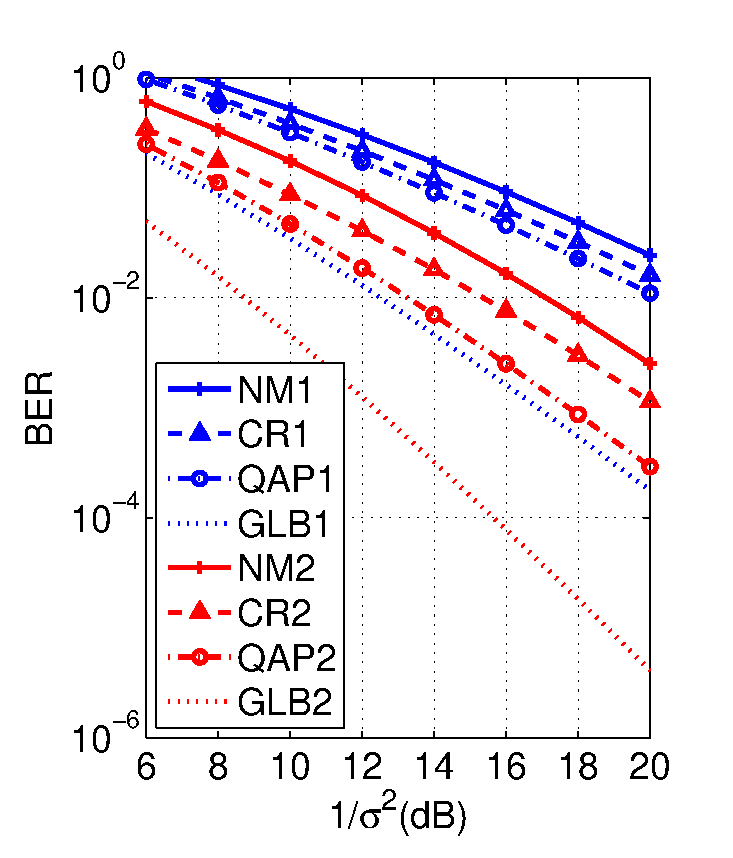
\includegraphics[width=4.5cm]{./figs/BER_noise_power_upperbound_64QAM_23.eps}}
    \centerline{(a) $m=1,2$}\medskip
  \end{minipage}
  \hfill
  \begin{minipage}[b]{0.48\linewidth}
    \centering
    \centerline{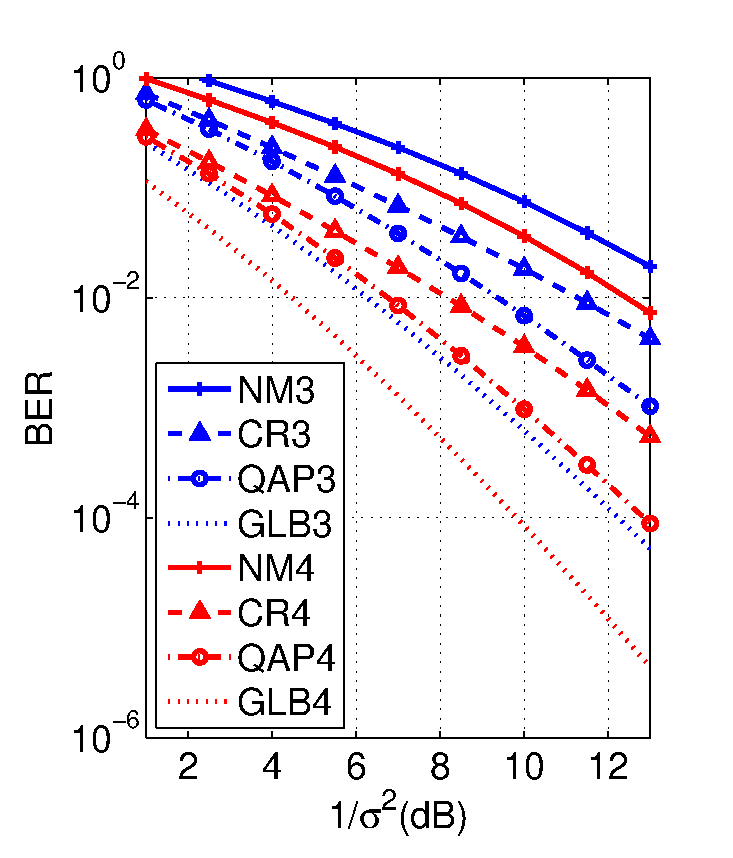
\includegraphics[width=4.5cm]{./figs/BER_noise_power_upperbound_64QAM_45.eps}}
    \centerline{(b) $m=3,4$}\medskip
  \end{minipage}
  \caption{The approximated uncoded BER.}
  \label{fig:uncoded_noisepower_approx}
\end{figure}

\begin{figure}[htb]
  \begin{minipage}[b]{.48\linewidth}
    \centering
    \centerline{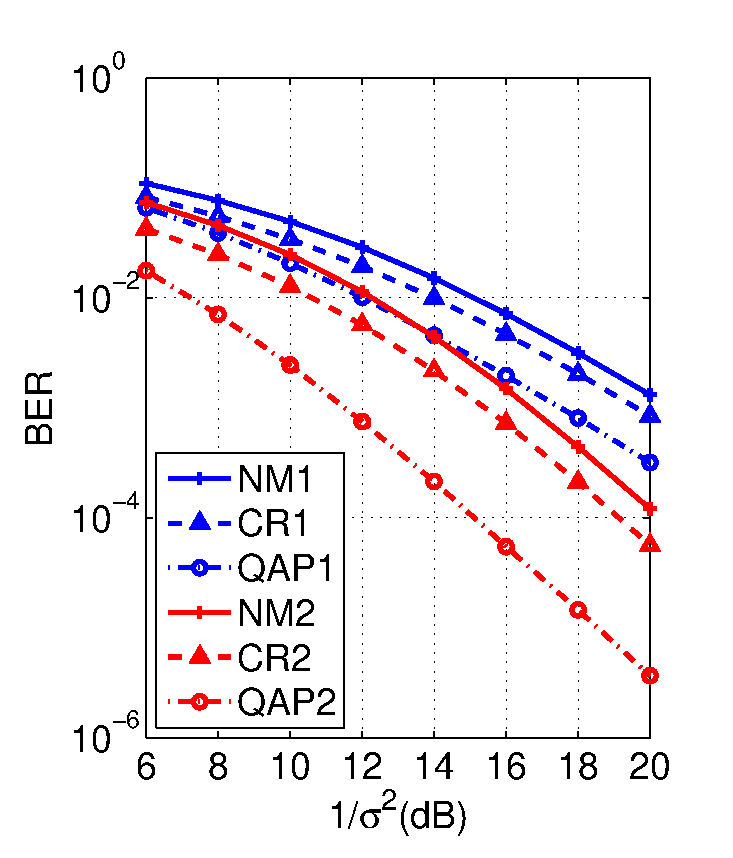
\includegraphics[width=4.5cm]{./figs/BER_noise_power_MonteCarlo_64QAM_23.eps}}
    \centerline{(a) $m=1,2$}\medskip
  \end{minipage}
  \hfill
  \begin{minipage}[b]{0.48\linewidth}
    \centering
    \centerline{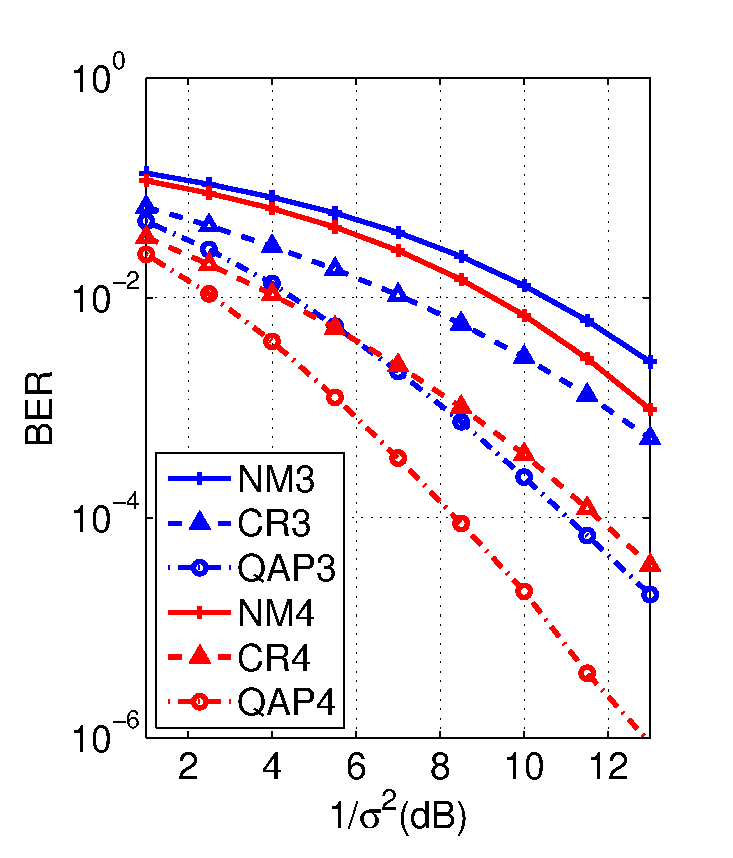
\includegraphics[width=4.5cm]{./figs/BER_noise_power_MonteCarlo_64QAM_45.eps}}
    \centerline{(b) $m=3,4$}\medskip
  \end{minipage}
  \caption{The Monte-Carlo simulated uncoded BER.}
  \label{fig:uncoded_noisepower_mc}
\end{figure}

To further verify the performance gain and robustness of the
QAP-optimized MoDiv scheme, we compare the coded-BER of the three MoDiv schemes
for 64-QAM constellation in a LDPC-coded communication system based
on~\cite{hochwald2003achieving}.
We use a LDPC code of length $L=2400$, coding rate of $3/4$ and a Monte-Carlo run
of up to 2000 LDPC frames. Since an important motivation of HARQ is to adopt for
link adaptation inaccuracies~\cite{cheng2006coding}, we deliberately optimize
the remappings at $\sigma^2=4.5dB$ and test their performances on
mismatching $\sigma^2$. The results are shown in
Fig.~\ref{fig:coded_64QAM_12} and Fig.~\ref{fig:coded_64QAM_34}. Apparently,
the advantage of QAP solution is preserved despite of mismatching. Specifically,
QAP2 still performs better than NM4, while CR4 outperforms QAP3 by less than
1dB.

% Coded BER for 16QAM for Non-MoDiv, Seddik, and QAP in one graph, M
% = 3, 4
\begin{figure}[htb]
  \centering
  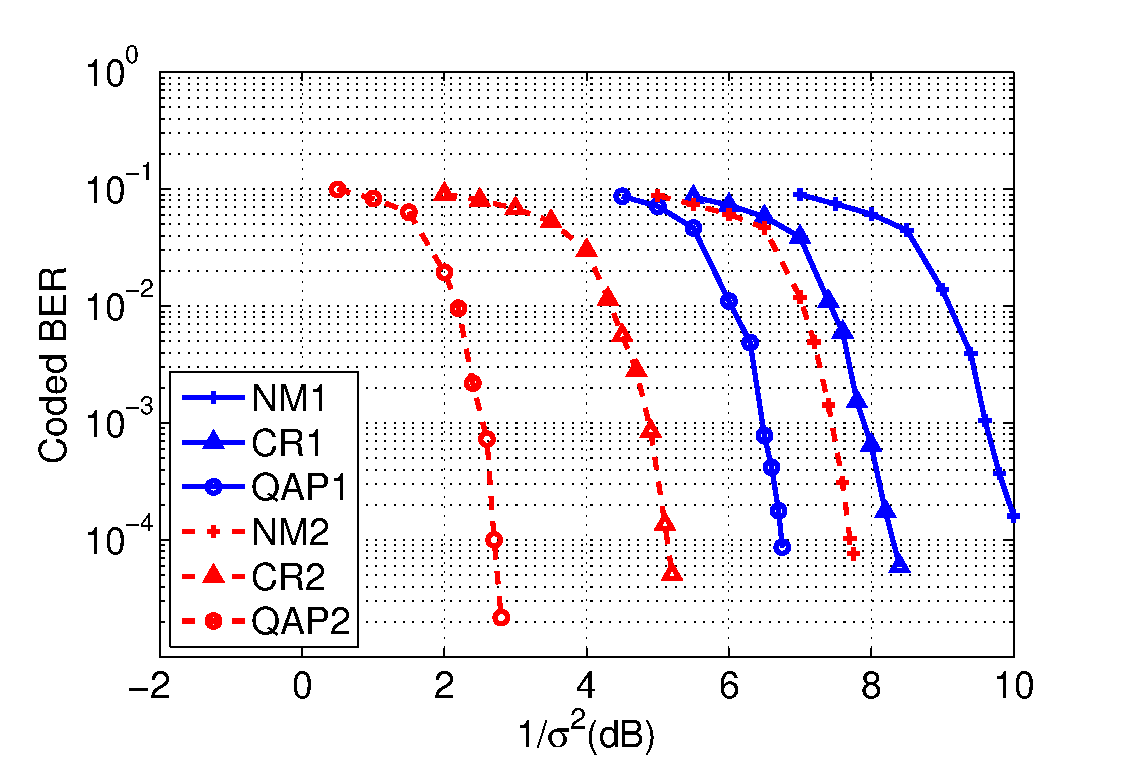
\includegraphics[width=0.9\columnwidth]{./figs/waterfall_2M3M_64QAM.eps}
  \caption{Coded BER for $m=1,2$.}
  \label{fig:coded_64QAM_12}
\end{figure}

% Coded BER for 64QAM for Non-MoDiv, Seddik, and QAP in one graph, M
% = 3, 4
\begin{figure}[htb]
  \centering
  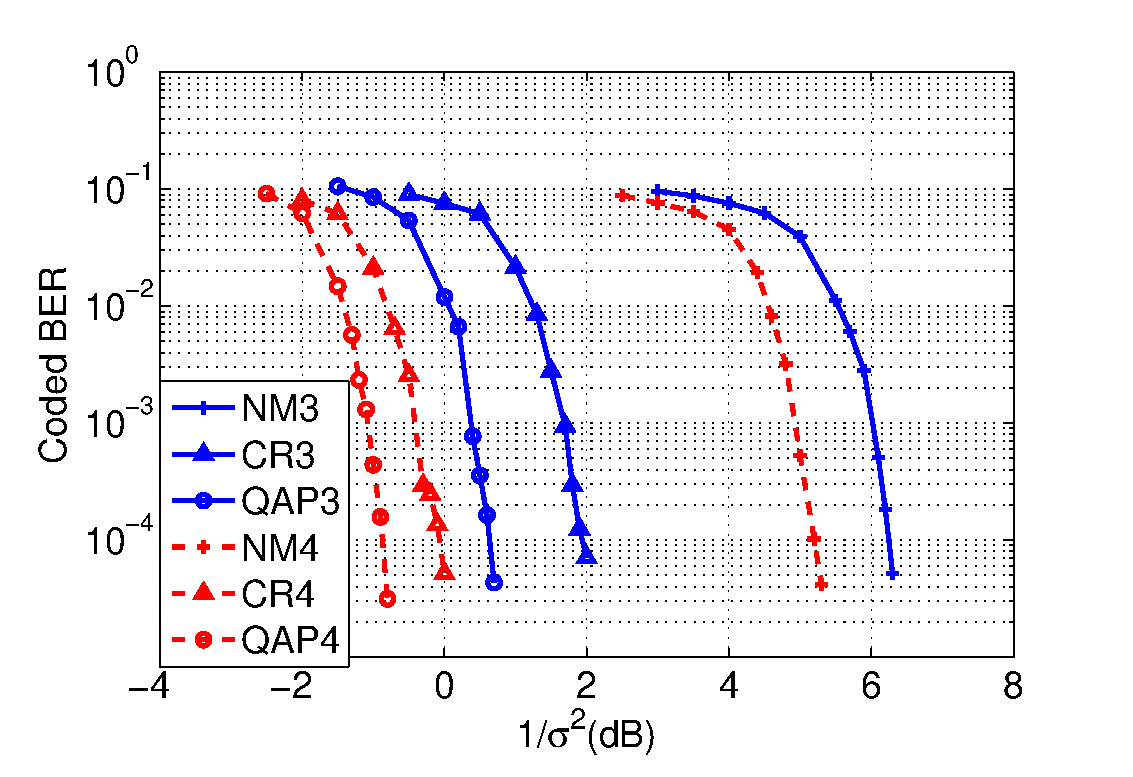
\includegraphics[width=0.9\columnwidth]{./figs/waterfall_4M5M_64QAM.eps}
  \caption{Coded BER for $m=3,4$.}
  \label{fig:coded_64QAM_34}
\end{figure}

Finally, to summarize the advantage of our QAP-based MoDiv scheme, we plot the
average HARQ throughput of the above LDPC coded system. For the 16-QAM result,
the QAP-based MoDiv design is solved at $\sigma^2=0dB$. It appears that
MoDiv design achieves greater performance gain for denser
constellation, since a larger space of constellation rearrangement offers more
opportunity to our QAP solver.

\begin{figure}[htb]
  \centering
  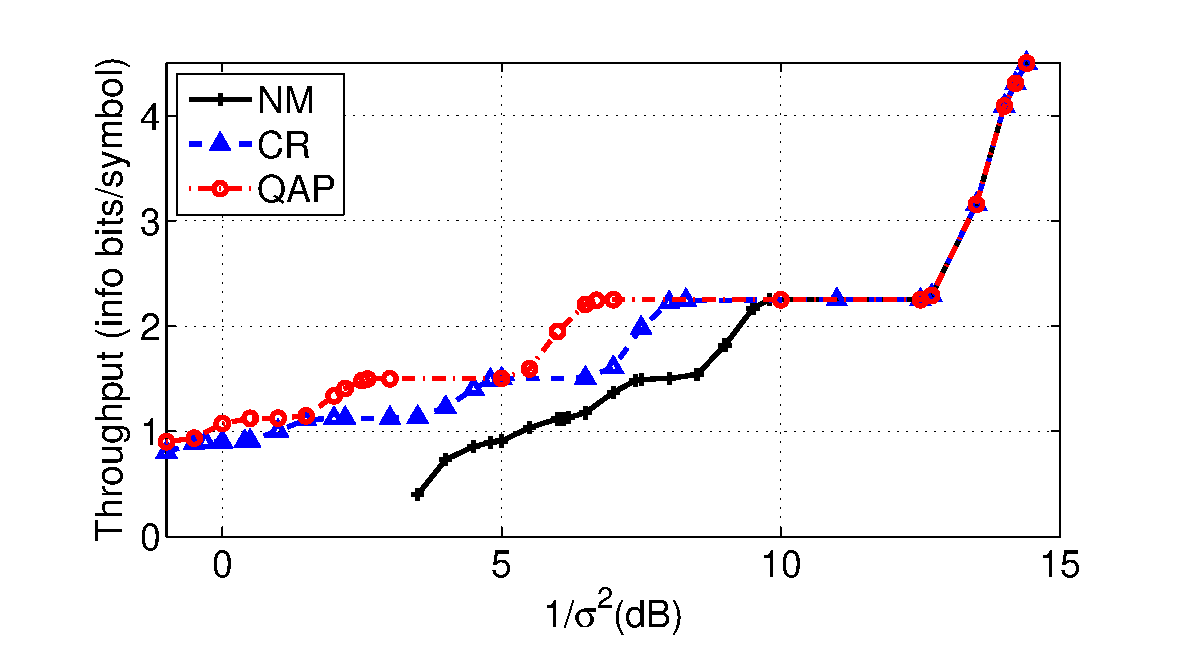
\includegraphics[width=0.9\columnwidth]{./figs/throughput_6M_64QAM.eps}
  \caption{Average throughput for 64-QAM.}
  \label{fig:coded_64QAM_12}
\end{figure}

\begin{figure}[htb]
  \centering
  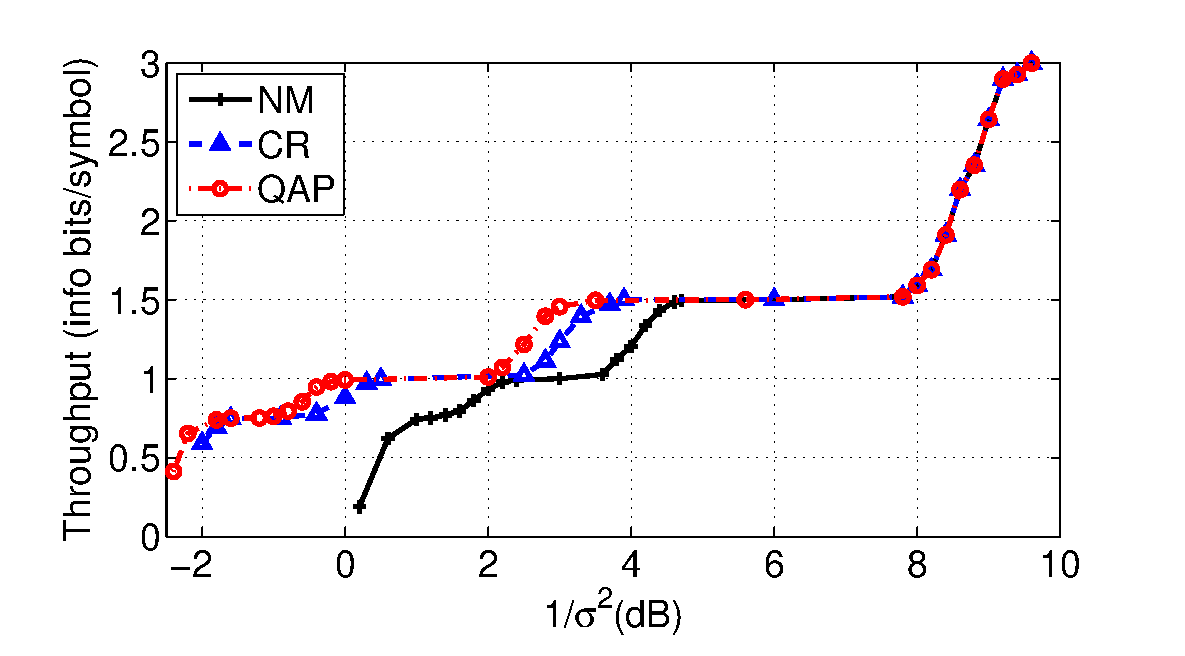
\includegraphics[width=0.9\columnwidth]{./figs/throughput_6M_16QAM.eps}
  \caption{Average throughput for 16-QAM.}
  \label{fig:coded_64QAM_12}
\end{figure}

\section{Conclusion}
\label{sec:conclusion}
In this work, we investigated the modulation diversity (MoDiv) design for
Chase Combining (CC) HARQ in amplify and forward (AF) two-way relay channel
(TWRC). With the objective of minimizing an approximated
bit error rate (BER), the MoDiv design was formulated into a successive
Koopmans-Beckmann Quadratic Assignment Problem (QAP) and solved with a robust
taboo search algorithm. Our numerical tests demonstrated that the QAP-optimized
MoDiv outperformed simple repeated use of Gray mapping and a heuristic
constellation rearrangement (CoRe) scheme under various settings and was robust
against mismatched design parameters.
% An example of a floating figure using the graphicx package.
% Note that \label must occur AFTER (or within) \caption.
% For figures, \caption should occur after the \includegraphics.
% Note that IEEEtran v1.7 and later has special internal code that
% is designed to preserve the operation of \label within \caption
% even when the captionsoff option is in effect. However, because
% of issues like this, it may be the safest practice to put all your
% \label just after \caption rather than within \caption{}.
%
% Reminder: the "draftcls" or "draftclsnofoot", not "draft", class
% option should be used if it is desired that the figures are to be
% displayed while in draft mode.
%
%\begin{figure}[!t]
%\centering
%\includegraphics[width=2.5in]{myfigure}
% where an .eps filename suffix will be assumed under latex, 
% and a .pdf suffix will be assumed for pdflatex; or what has been declared
% via \DeclareGraphicsExtensions.
%\caption{Simulation results for the network.}
%\label{fig_sim}
%\end{figure}

% Note that IEEE typically puts floats only at the top, even when this
% results in a large percentage of a column being occupied by floats.


% An example of a double column floating figure using two subfigures.
% (The subfig.sty package must be loaded for this to work.)
% The subfigure \label commands are set within each subfloat command,
% and the \label for the overall figure must come after \caption.
% \hfil is used as a separator to get equal spacing.
% Watch out that the combined width of all the subfigures on a 
% line do not exceed the text width or a line break will occur.
%
%\begin{figure*}[!t]
%\centering
%\subfloat[Case I]{\includegraphics[width=2.5in]{box}%
%\label{fig_first_case}}
%\hfil
%\subfloat[Case II]{\includegraphics[width=2.5in]{box}%
%\label{fig_second_case}}
%\caption{Simulation results for the network.}
%\label{fig_sim}
%\end{figure*}
%
% Note that often IEEE papers with subfigures do not employ subfigure
% captions (using the optional argument to \subfloat[]), but instead will
% reference/describe all of them (a), (b), etc., within the main caption.
% Be aware that for subfig.sty to generate the (a), (b), etc., subfigure
% labels, the optional argument to \subfloat must be present. If a
% subcaption is not desired, just leave its contents blank,
% e.g., \subfloat[].


% An example of a floating table. Note that, for IEEE style tables, the
% \caption command should come BEFORE the table and, given that table
% captions serve much like titles, are usually capitalized except for words
% such as a, an, and, as, at, but, by, for, in, nor, of, on, or, the, to
% and up, which are usually not capitalized unless they are the first or
% last word of the caption. Table text will default to \footnotesize as
% IEEE normally uses this smaller font for tables.
% The \label must come after \caption as always.
%
%\begin{table}[!t]
%% increase table row spacing, adjust to taste
%\renewcommand{\arraystretch}{1.3}
% if using array.sty, it might be a good idea to tweak the value of
% \extrarowheight as needed to properly center the text within the cells
%\caption{An Example of a Table}
%\label{table_example}
%\centering
%% Some packages, such as MDW tools, offer better commands for making tables
%% than the plain LaTeX2e tabular which is used here.
%\begin{tabular}{|c||c|}
%\hline
%One & Two\\
%\hline
%Three & Four\\
%\hline
%\end{tabular}
%\end{table}


% Note that the IEEE does not put floats in the very first column
% - or typically anywhere on the first page for that matter. Also,
% in-text middle ("here") positioning is typically not used, but it
% is allowed and encouraged for Computer Society conferences (but
% not Computer Society journals). Most IEEE journals/conferences use
% top floats exclusively. 
% Note that, LaTeX2e, unlike IEEE journals/conferences, places
% footnotes above bottom floats. This can be corrected via the
% \fnbelowfloat command of the stfloats package.



% if have a single appendix:
%\appendix[]

% or
%\appendix  % for no appendix heading
% do not use \section anymore after \appendix, only \section*
% is possibly needed

% use appendices with more than one appendix
% then use \section to start each appendix
% you must declare a \section before using any
% \subsection or using \label (\appendices by itself
% starts a section numbered zero.)
%


\appendices
\section{Proof of Proposition~\ref{prop:E_k}}
\label{sec:appenda}
The proof of Proposition~\ref{prop:E_k} is generally based on Eq.(43)
of~\cite{han2009performance}. Firstly, by adopting the heuristic approximation
in~\cite{jing2006distributed}, the random variable $\alpha^{(k)}$ is replaced
with constant $\tilde{\alpha}$ in $E_k[p, q]$, then we have
\begin{align}
  E_k[p, q] & \approx \mathbb{E}_{\gamma_2}
  \left[
  \mathbb{E}_{\delta_1|\gamma_2}
  \left[
  \exp\left(
  -\frac{\tilde{\alpha}^2\epsilon_k[p,q]\gamma_2 \delta_1}
  {4(\sigma_2^2+\tilde{\alpha}^2\sigma_R^2\gamma_2)}
  \right)
  \right]
  \right] \notag \\
  & = \mathbb{E}_{\gamma_2}
  \left[
  \left(1 + \frac{\tilde{\alpha}^2\epsilon_k[p,q]\beta_{h_1}\gamma_2 }
  {4(\sigma_2^2+\tilde{\alpha}^2\sigma_R^2\gamma_2)}\right)^{-1}
  \right]. \label{eq:ekpq_approx}
\end{align}
As $\delta_1,\gamma_2$ both follow exponential distribution,
Eq.(\ref{eq:E_k}) is derived by evaluating Eq.(\ref{eq:ekpq_approx}) with
Eq.(3.352.4) of~\cite{zwillinger2014table}.


\section{Proof of Proposition~\ref{prop:EMI}}
\label{sec:appendb}
Denote the mutual information conditioned on the channel state
informations as $I^{(m)}(\mathbf{h}_1^{(m)}, \mathbf{g}_2^{(m)},
\bm{\alpha}^{(m)})$, where $\mathbf{h}_1^{(m)} =
[h_1^{(0)},\ldots,h_1^{(m)}]^T$, $\mathbf{g}_2^{(m)} =
[g_2^{(0)},\ldots,g_2^{(m)}]^T$ and $\bm{\alpha}^{(m)} =
[\alpha^{(0)},\ldots,\alpha^{(m)}]^T$. By assuming a
uniform distribution of all constellation symbols, $I^{(m)}(\mathbf{h}_1^{(m)},
\mathbf{g}_2^{(m)}, \bm{\alpha}^{(m)})$ is lower bounded with~\cite[Eq.(4.3.37)]{}:
\begin{align}
  & \tilde{I}^{(m)}(\mathbf{h}_1^{(m)}, \mathbf{g}_2^{(m)},
  \bm{\alpha}^{(m)}) = \log_2Q - \notag \\
  & \log_2\left[\frac{1}{Q} \sum_{p=0}^{Q-1}\sum_{q=0}^{Q-1}
  \prod_{k=0}^{m}\exp\left(-
  \frac{(\alpha^{(k)})^2\epsilon_k[p,q]\gamma_2^{(k)}\delta_1^{(k)}}
  {4(\tilde{\sigma}_2^{(k)})^2} \right) \right].
\end{align}
Noting that $\log(x)$ is a concave function
and the channels are assumed independent across each round of
(re)transmissions, we have $\mathbb{E}\left[\tilde{I}^{(m)}(\mathbf{h}_1^{(m)},
\mathbf{g}_2^{(m)}, \bm{\alpha}^{(m)})\right] \geq \tilde{I}^{(m)}$, thus
Proposition~\ref{prop:EMI} is proved.
%Appendix one text goes here.

% you can choose not to have a title for an appendix
% if you want by leaving the argument blank
%\section{}
%Appendix two text goes here.


% use section* for acknowledgment
%\section*{Acknowledgment}


%The authors would like to thank...


% Can use something like this to put references on a page
% by themselves when using endfloat and the captionsoff option.
\ifCLASSOPTIONcaptionsoff
  \newpage
\fi



% trigger a \newpage just before the given reference
% number - used to balance the columns on the last page
% adjust value as needed - may need to be readjusted if
% the document is modified later
%\IEEEtriggeratref{8}
% The "triggered" command can be changed if desired:
%\IEEEtriggercmd{\enlargethispage{-5in}}

% references section

% can use a bibliography generated by BibTeX as a .bbl file
% BibTeX documentation can be easily obtained at:
% http://www.ctan.org/tex-archive/biblio/bibtex/contrib/doc/
% The IEEEtran BibTeX style support page is at:
% http://www.michaelshell.org/tex/ieeetran/bibtex/
\bibliographystyle{IEEEtran}
% argument is your BibTeX string definitions and bibliography database(s)
\bibliography{IEEEabrv,./refs.bib}

%
% <OR> manually copy in the resultant .bbl file
% set second argument of \begin to the number of references
% (used to reserve space for the reference number labels box)
%\begin{thebibliography}{1}

%\bibitem{IEEEhowto:kopka}
%H.~Kopka and P.~W. Daly, \emph{A Guide to \LaTeX}, 3rd~ed.\hskip 1em plus
%  0.5em minus 0.4em\relax Harlow, England: Addison-Wesley, 1999.

%\end{thebibliography}

% biography section
% 
% If you have an EPS/PDF photo (graphicx package needed) extra braces are
% needed around the contents of the optional argument to biography to prevent
% the LaTeX parser from getting confused when it sees the complicated
% \includegraphics command within an optional argument. (You could create
% your own custom macro containing the \includegraphics command to make things
% simpler here.)
%\begin{IEEEbiography}[{\includegraphics[width=1in,height=1.25in,clip,keepaspectratio]{mshell}}]{Michael Shell}
% or if you just want to reserve a space for a photo:

%\begin{IEEEbiography}{Michael Shell}
%Biography text here.
%\end{IEEEbiography}

% if you will not have a photo at all:
%\begin{IEEEbiographynophoto}{John Doe}
%Biography text here.
%\end{IEEEbiographynophoto}

% insert where needed to balance the two columns on the last page with
% biographies
%\newpage

%\begin{IEEEbiographynophoto}{Jane Doe}
%Biography text here.
%\end{IEEEbiographynophoto}

% You can push biographies down or up by placing
% a \vfill before or after them. The appropriate
% use of \vfill depends on what kind of text is
% on the last page and whether or not the columns
% are being equalized.

%\vfill

% Can be used to pull up biographies so that the bottom of the last one
% is flush with the other column.
%\enlargethispage{-5in}



% that's all folks
\end{document}


